\question{Действие сил пространственного заряда на траекторию крайнего электрона
  в цилиндрическом электронном потоке}

Рассмотрим движение потока кругового поперечного сечения радиуса \( R_0 \) в 
эквипотенциальной области, где на него не действуют никакие внешние силы. 
Потенциал в области \( U_0 \), \( I_0 \) -- ток пучка. Считаем, что все 
электроны имеют одинаковую продольную скорость \( v_{0z} \approx v_0 \), 
плотность тока одинакова во всех точках каждого поперечного сечения, но каждый 
электрон потока обладает радиальной скоростью.

Для определения траекторий электронов необходимо знать все составляющие 
напряженности электростатического поля, вызванные взаимодействием соседних частиц.

Поскольку пучок имеет цилиндрическую форму, то он имеет только \( E_r \) -- 
составляющую поля пространственного заряда:
\begin{equation}
	E_r = \frac{\tau}{2\pi\eps_0 r}
	\label{eq13.3.17}
\end{equation}
где \( \tau \) -- линейная плотность пространственного заряда.

Если известен ток \( I_0 \), то линейная плотность заряда в пучке:
\[
	\tau = 2\pi r^2 \rho = -\frac{j}{v_0}2\pi r^2 = -\frac{I_0}{v_0}
\]
Подставляя это выражение в (\ref{eq13.3.17}), находим выражение для радиальной 
составляющей напряженности поля пространственного заряда:
\begin{equation}
	E_r = -\frac{I_0}{2\pi\eps_0 v_0 r}
	\label{eq13.3.18}
\end{equation}
 
Движение электронов пучка состоит из двух составляющих: вдоль оси пучка 
(\( dz/dt = v_0\)) и в радиальном направлении
\begin{equation}
	\ddot{r} = -\left| \frac{e}{m} \right|E_r
	\label{eq13.3.19}
\end{equation}

Для анализа траекторий перейдем к уравнению в плоскости, воспользовавшись 
соотношением \( \ddot{r} = 2\left| e/m \right| U_0 \frac{d^2 r}{dz^2} \), где 
\( U_0 \) -- потенциал, соответствующий скорости движения электронов 
\( v_0 \). Тогда  уравнение (\ref{eq13.3.19}) принимает вид
\begin{equation}
	\frac{d^2 r}{dz^2} = 
		-\frac{1}{4\pi\eps_0 \sqrt{2\left|\frac{e}{m}\right|}}
		\frac{I_0}{U_0^{3/2}}\frac{1}{r}
	\label{eq13.3.20}
\end{equation}
 
Учитывая (\ref{eq12.3.13}) и обозначая 
\[
	\alpha = \frac{P}{2\pi\eps_0 \sqrt{2\left|\frac{e}{m}\right|}}
\]
преобразуем уравнение траекторий к виду
\begin{equation}
	\frac{d^2 r}{dz^2} = \frac{\alpha}{2r}
	\label{eq13.3.21}
\end{equation}
 
Для удобства расчета введем безразмерные переменные \( R = r/r_0 \); 
\( Z = \alpha^{1/2}(z/r_0) \) и произведем замену \( r \) и \( z \) в 
(\ref{eq13.3.21}):
\begin{equation}
	\frac{d^2 R}{dZ^2} = \frac{1}{2R}
	\label{eq13.3.22}
\end{equation}
Используя то, что \( \cfrac{d}{dZ}(R')^2 = 2R'R'' \) (штрихи означают первую 
и вторую производные по \( z \), то есть 
\( R'' = \cfrac{d^2 R}{dZ^2} = \cfrac{1}{2R'}\cfrac{d}{dZ}(R')^2 \), после 
подстановки в (\ref{eq13.3.22}) получаем:
\[
	\frac{d^2 R}{dZ^2} = \frac{1}{2R'}\frac{d}{dZ}(R')^2 = \frac{1}{2R}
	\text{, или } \frac{d}{dZ}(R')^2 = \frac{d}{dZ}(\ln R)
\]

В результате интегрирования
\begin{equation}
	\left( \frac{dR'}{dZ} \right)^2 = \ln R + (R'_0)^2
	\label{eq13.3.23}
\end{equation}
 
где \( R'_0 \) -- постоянная интегрирования, определяемая из условий на 
границе влета пучка в исследуемое пространство: при \( z = 0 \) 
\( \frac{dR}{dZ} = \tg\gamma_0 \) -- угол наклона траектории электрона. Тогда 
\( R'_0 = \tg\gamma_0 \).

Из (\ref{eq13.3.23}) при \( R' = 0 \) можно определить минимальное значение 
\( R \):
\begin{equation}
	R_{min} = \exp\left[ -(R'_0)^2 \right]
	\label{eq13.3.24}
\end{equation}
Для определения истинных траекторий введем новую переменную \( u = dR/dZ \).
Тогда, поскольку \( \ln R = (R')^2 - (R'_0)^2 \); 
\( R = \exp\left[ -(R'_0)^2 \right] e^{u^2} \); и 
\[
	\frac{dR}{dZ} = u = 2 \exp\left[ -(R'_0)^2 \right] ue^{u^2} \frac{du}{dZ}
\]
Отсюда получаем соотношение 
\( dZ = 2 \exp\left[ -(R'_0)^2 \right] e^{u^2} du \), а после интегрирования -- 
траекторию:
\begin{equation}
	Z = 2\exp\left[ -(R'_0)^2 \right] 
		\int\limits_{R'_0}^{\pm\sqrt{ln R+(R'_0)^2}} e^{u^2} di
	\label{eq13.3.25}
\end{equation}

Пределы интегрирования выбираются из следующих соображений. Для пучка, у 
которого \( R'_0 < 0 \) и \( R_0 < 1 \)  (сходящийся на входе пучка), в
верхнем пределе надо брать знак минус. В этом случае уравнение 
(\ref{eq13.3.25}) описывает траекторию крайнего электрона на участке от 
\( z = 0 \) до точки, где \( R = R_{min} \), а \( Z = Z_{min} \) (до плоскости 
кроссовера). Для пучка, длина которого больше  \( Z_{min} \) и \( R' > 0 \), в 
верхнем пределе берется знак плюс.
\begin{figure}[h!]
	\center
	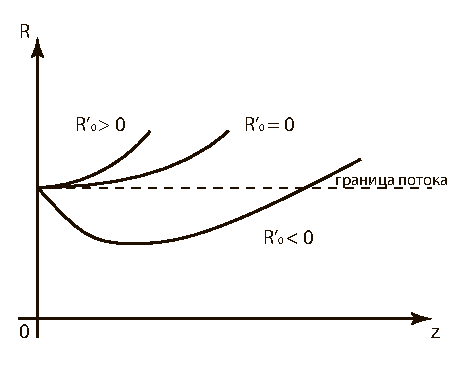
\includegraphics[width=.4\textwidth]{13_1}
	\caption{Контур границы цилиндрического 
		электронного потока при учёте полей пространственного заряда}
	\label{img13.1}
\end{figure}

На рис.\ref{img13.1} приведены графики траекторий крайних электронов потока 
при различных \( R'_0 < 0 \). Из них видно, что существует вполне определенный 
угол встрела граничных электронов, обеспечивающий максимальную длину пролета 
пучка по каналу радиуса \( R = 1 \). Этот угол, согласно расчетам, 
приближенно можно оценить по соотношению \( \tg\gamma_{opt} = -162\sqrt{P} \). 
При этом расстояние до плоскости кроссовера равно:
\( Z_{opt} = r(0)\left| \tg\gamma_{opt} \right|^{-1} \).